

\section{T-Beams}

\begin{figure}[h]
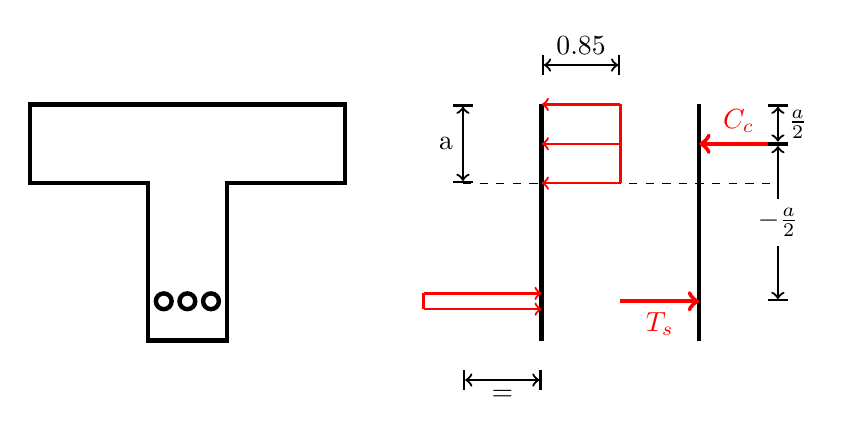
\begin{tikzpicture}
	
	
	\begin{scope}
	
	\pgfmathsetmacro{\be}{4}
	\pgfmathsetmacro{\H}{3}
	\pgfmathsetmacro{\hf}{1}
	
	\coordinate (A) at (0, \H);
	\coordinate (B) at (\be,\H);
	\coordinate (C) at (\be,\H-\hf);
	\coordinate (D) at (2.5,\H-\hf);
	\coordinate (E) at (2.5,0);
	\coordinate (F) at (1.5,0);
	\coordinate (G) at (1.5,2);
	\coordinate (H) at (0,2);
	
	\draw[ultra thick] 
		(A) -- 
		(B) -- 
		(C) --
		(D) -- 
		(E) -- 
		(F) -- 
		(G) -- 
		(H) --
		cycle;
	
	\draw[ultra thick,fill=white] (2,0.5) circle (0.1cm);
	\draw[ultra thick,fill=white] (2.3,0.5) circle (0.1cm);
	\draw[ultra thick,fill=white] (1.7,0.5) circle (0.1cm);
	\end{scope}
	

	
	\begin{scope}[xshift=-0.5cm]
	%% Stress axis line
	\draw[ultra thick] (7,0) -- (7,3);
	\draw[thick,|<->|] (6,2) -- node[left]{a} (6,3);
	\draw[thin, dashed] (6,2) -- (10,2);
	
	\draw[thick,|<->|] (7,3.5) -- node[above]{0.85\fc} (8,3.5);
	\draw[thick,|<->|] (6,-0.5) -- node[below]{\fs=\fy} (7,-0.5);
	
	%whitney stress block arrows
	\draw[thick,red,->] (8,3) -- (7,3);
	\draw[thick,red,->] (8,2.5) -- (7,2.5);
	\draw[thick,red,->] (8,2) -- (7,2);
	\draw[thick, red] (8,3) -- (8,2);
	
	% Steel stress
	\draw[thick, red, <-] (7,0.6) -- (5.5,0.6);
	\draw[thick, red, <-] (7,0.4) -- (5.5,0.4);
	\draw[thick, red] (5.5,0.4) -- (5.5,0.6);
	\end{scope}
	
	\begin{scope}[xshift=-0.5cm]
	%% Force axis line
	\draw[ultra thick] (9,0) -- (9,3);
	
	% Resultant forces
	% Comression
	\draw[ultra thick, red, <-] (9,2.5) -- node[above,fill=white]{$C_c$} (10,2.5);
	\draw[thick, |<->|] (10,2.5) -- node[right]{$\frac{a}{2}$} (10,3);
	%Tension
	\draw[ultra thick, red, ->] (8,0.5) -- node[below,fill=white]{$T_s$} (9,0.5);
	
	\draw[thick, |<->|] (10,2.5) -- node[fill=white]{$\dd-\frac{a}{2}$} (10,0.5);
	
	\end{scope}
	
\end{tikzpicture}
\end{figure}